\section[MEX 2-4: Large wellbore test (Springen)]{Model-Experiment-Exercise 2-4:\\Large wellbore test (Springen)}
\label{sec:mex11}
\index{URL Springen}
%------------------------------------------------------------------------------
\Authors{Mathias Nest}
%------------------------------------------------------------------------------

\begin{figure}[ht]
\centering
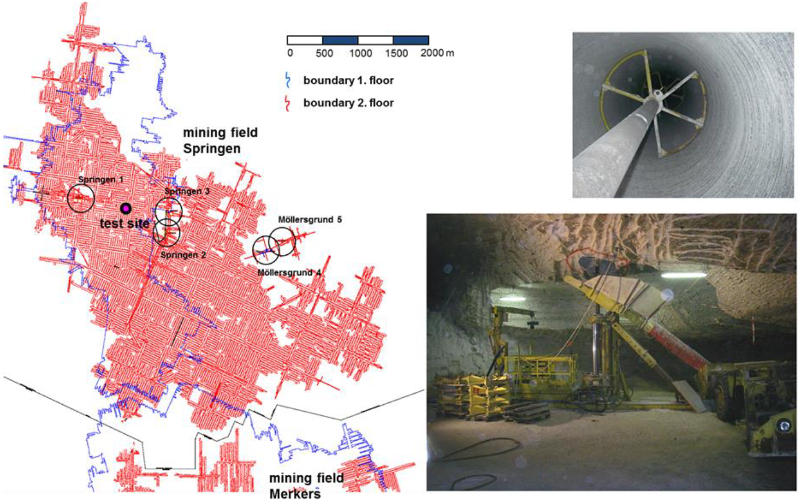
\includegraphics[width=0.9\textwidth]{figures/IfG-borehole-overview-small.png}
\caption{Mining field Springen (left), borehole (right)}
\label{fig:largeborehole1}
\end{figure}

The motivation for this experiment was two-fold. First, decommissioned caverns are usually filled with brine before they are closed and sealed. The lower density of the brine leads to a buoyant force, so that the pressure in the liquid can become larger than the lithostatic stress in that depth. This led to questions about the long-term tightness of abandoned caverns, and thus safety concerns. Of central importance was the question, whether a large, long-range frac would be suddenly created, or a slow expansion between the salt crystals would take place. 

\begin{figure}[ht]
\centering
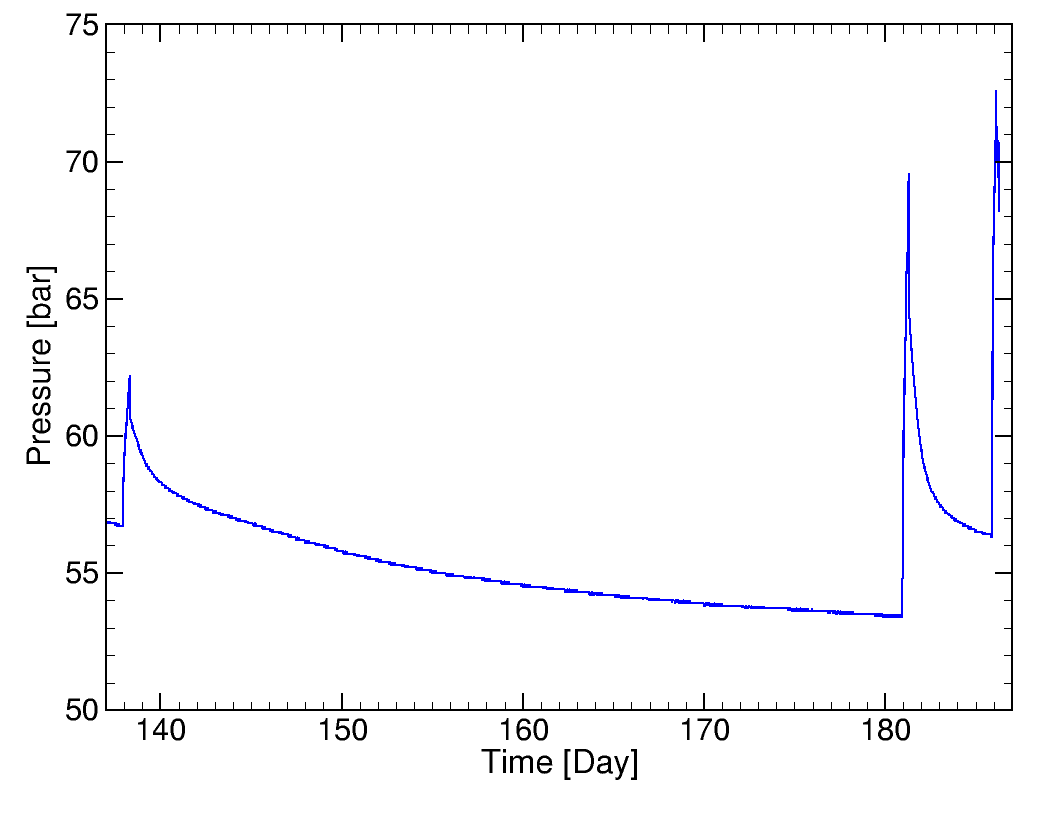
\includegraphics[width=0.8\textwidth]{figures/IfG-Druckkurve-50d.png}
\caption{Sequence of three pressure applications over a span of 50 days.}
\label{fig:largeborehole2}
\end{figure}

Second, from a scientific point of view, it is interesting to see whether there is a difference in the pressure driven percolation between liquids and gases. To conduct experiments under realistic in situ conditions to answer these questions a large borehole with a volume of about 50 m$^3$ was excavated between two seams in the Springen mining field, see also Sec. \ref{sec:springen} and Fig. \ref{fig:largeborehole1}. In 2011/2012 this borehole was used to conduct an experiment with pressurized air. Here, we report results of an experiment performed in 2018, where the borehole was loaded with brine. Starting in early 2018, the brine pressure was increased in small steps of around 5 bar, followed by periods of rest, where the surrounding rock was allowed to react. In the summer a pressure level was reached that was close to the minimal principal stress of about 50 bar. Fig. \ref{fig:largeborehole2} shows the last three pressure spikes over a span of 50 days. They were created by pumping brine with rates of 2 l/h, 3.3 l/h and 5.5 l/h, respectively. Each time, a rapid drop in pressure was observed consistent with the high bulk modulus of brine and the simulations in Sec. \ref{sec:mex04}. The fact that more than 60 bar were required to induce cracks between salt crystals, i.e. more than minimal principal stress, is due to the tensile/adhesive strength of rock salt. 

The central part of the figure shows, that the decay of the pressure still continues 6 weeks after the pressure spike, showing the slow expansion of the brine into the surrounding area. The final spike was an attempt to determine the highest pressure obtainable with available equipment (however, with the previously damaged rock salt). The experiment ended August 14, 2018. Acoustic emission data has been collected, but requires further analysis. Further pressure measurements in the spring of 2019 provided values of around 50 bar, consistent with the minimal stress criterion. 

